\documentclass[12pt,a4paper]{article}
\usepackage{fontspec}
\setmainfont{TeX Gyre Termes}
\usepackage[a4paper,margin=2.2cm]{geometry}
\usepackage{graphicx}
\usepackage{float}
\usepackage{booktabs}
\usepackage{longtable}
\usepackage{array}
\usepackage{fancyhdr}
\usepackage{hyperref}
\usepackage{amsmath}
\usepackage{enumitem}
\hypersetup{colorlinks=true, linkcolor=blue, urlcolor=blue}
\setlength{\parindent}{0pt}
\setlength{\parskip}{6pt}
\renewcommand{\arraystretch}{1.25}
\setlength{\headheight}{15pt}

\pagestyle{fancy}
\fancyhf{}
\fancyfoot[C]{\thepage}
\renewcommand{\headrulewidth}{0pt}

\begin{document}

\begin{titlepage}
    \thispagestyle{empty}
    \centering

    \vspace*{1.5cm}
    
\includegraphics[width=3.2cm]{../../../../../assets/rsz_logo-khtn.png}\par
    \vspace{0.8cm}

    {\Large\bfseries ĐẠI HỌC QUỐC GIA THÀNH PHỐ HỒ CHÍ MINH\par}
    \vspace{0.2cm}
    {\Large\bfseries TRƯỜNG ĐẠI HỌC KHOA HỌC TỰ NHIÊN\par}
    \vspace{0.15cm}
    {\large KHOA CÔNG NGHỆ THÔNG TIN\par}

    \vspace{2.0cm}
    {\Large\bfseries BÁO CÁO THỰC HÀNH 02\par}
    \vspace{0.4cm}
    {\large\bfseries Làm trơn ảnh và phát hiện biên cạnh\par}

    \vspace{1.8cm}
    \begin{tabular}{>{\bfseries}l l}
        Nhóm: & Myopia \\
        MSHV 1: & 25C11067 - Nguyễn Thái Thông \\
        MSHV 2: & 25C11035 - Trần Hạ Khánh Duy
    \end{tabular}

    \vfill
    {\large TP. Hồ Chí Minh, 2026\par}
\end{titlepage}
\clearpage
\pagenumbering{arabic}

\section{Mục tiêu}

Bài thực hành gồm hai nhóm nội dung chính: làm trơn ảnh và phát hiện biên cạnh. Phần làm trơn ảnh cài đặt và so sánh các bộ lọc mean filter, Gaussian filter và median filter. Phần phát hiện biên cạnh cài đặt và so sánh Sobel, Laplacian, Laplace of Gaussian (LoG) và Canny. Mỗi thuật toán được thực hiện bằng hai cách: cài đặt thủ công và dùng hàm OpenCV, sau đó đánh giá bằng hình minh chứng, MSE, thời gian chạy và bộ nhớ sử dụng.

\section{Phân công đóng góp}

\begin{longtable}{p{0.16\textwidth}p{0.26\textwidth}p{0.46\textwidth}p{0.10\textwidth}}
\toprule
\textbf{MSHV} & \textbf{Họ tên} & \textbf{Công việc} & \textbf{Tỉ lệ} \\
\midrule
25C11067 & Nguyễn Thái Thông & Cài đặt mean filter, Gaussian filter, Sobel; xây dựng hàm đo thời gian/bộ nhớ, kiểm thử kết quả thủ công so với OpenCV, thu thập hình minh chứng cho phần làm trơn và Sobel. & 50\% \\
25C11035 & Trần Hạ Khánh Duy & Cài đặt median filter, Laplacian, LoG, Canny; tổng hợp số liệu MSE, nhận xét kết quả, lưu output, hoàn thiện notebook và viết báo cáo. & 50\% \\
\bottomrule
\end{longtable}

\section{Bảng tự đánh giá}

\begin{longtable}{p{0.74\textwidth}>{\centering\arraybackslash}p{0.22\textwidth}}
\toprule
\textbf{Nội dung} & \textbf{Mức độ hoàn thành} \\
\midrule
Chuẩn bị môi trường, tải ảnh Lenna và hiển thị ảnh & 100\% \\
Làm trơn ảnh bằng mean filter & 100\% \\
Làm trơn ảnh bằng Gaussian filter & 100\% \\
Làm trơn ảnh bằng median filter & 100\% \\
Phát hiện biên cạnh bằng LoG & 100\% \\
Phát hiện biên cạnh bằng Sobel & 100\% \\
Phát hiện biên cạnh bằng Laplacian & 100\% \\
Phát hiện biên cạnh bằng Canny & 100\% \\
So sánh với hàm OpenCV & 100\% \\
Thu thập hình minh chứng và lưu kết quả & 100\% \\
Báo cáo & 100\% \\
\bottomrule
\end{longtable}

\section{Cơ sở lý thuyết tóm tắt}

\subsection{Làm trơn ảnh}

Làm trơn ảnh là bước tiền xử lý dùng để giảm nhiễu hoặc giảm các chi tiết nhỏ trong ảnh. Bộ lọc trung bình thay mỗi pixel bằng giá trị trung bình của vùng lân cận nên làm mờ đều. Bộ lọc Gaussian dùng trọng số lớn hơn cho các điểm gần tâm kernel, vì vậy ảnh sau lọc thường tự nhiên hơn so với mean filter. Bộ lọc median thay pixel bằng trung vị của vùng lân cận, phù hợp khi ảnh có nhiễu dạng điểm hoặc nhiễu muối tiêu.

\subsection{Phát hiện biên cạnh}

Biên cạnh là vùng có thay đổi cường độ sáng mạnh. Sobel dùng đạo hàm bậc một theo hai hướng $x$ và $y$, sau đó tính độ lớn gradient. Laplacian dùng đạo hàm bậc hai nên nhạy với các vùng biến thiên mạnh nhưng cũng dễ bị ảnh hưởng bởi nhiễu. Canny là phương pháp nhiều bước gồm làm trơn Gaussian, tính gradient, non-maximum suppression, ngưỡng kép và nối biên bằng hysteresis.

\section{Đánh giá kết quả}

\subsection{Ảnh đầu vào}

Ảnh Lenna được tải và resize về kích thước nhỏ hơn để các thuật toán thủ công chạy nhanh. Ảnh màu được chuyển sang ảnh xám trước khi áp dụng các thuật toán phát hiện biên.

\begin{figure}[H]
    \centering
    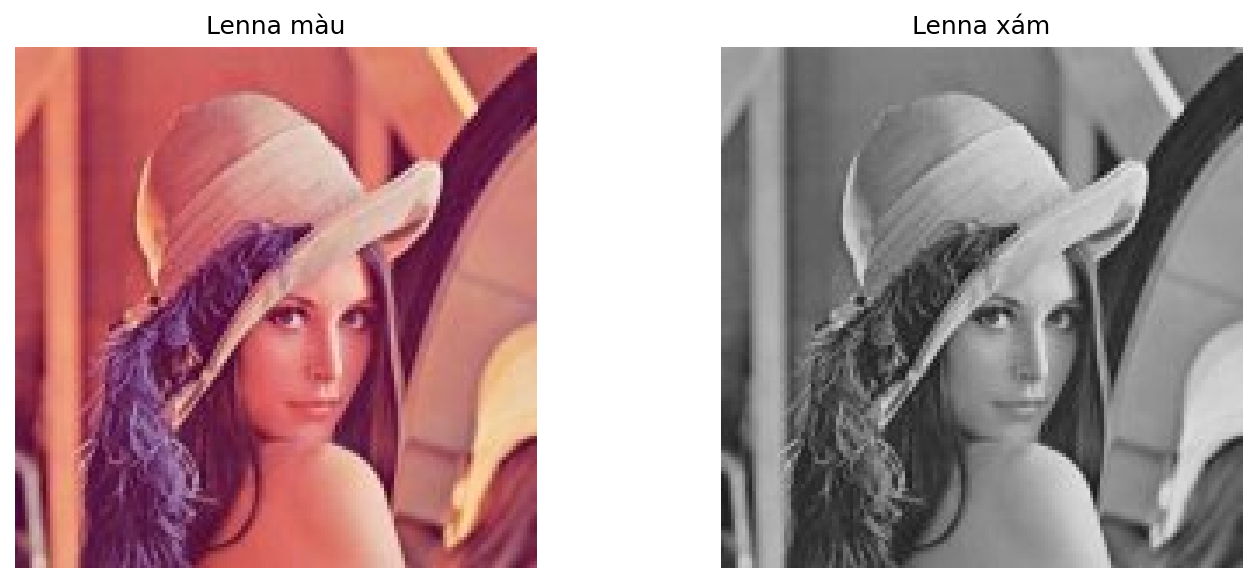
\includegraphics[width=0.80\textwidth]{figures/01_lenna.png}
    \caption{Ảnh Lenna màu và ảnh Lenna xám.}
\end{figure}

\subsection{Làm trơn ảnh}

Mean filter làm giảm nhiễu bằng cách lấy trung bình các pixel trong vùng lân cận. Trong notebook, nhóm hiển thị thêm ảnh sai khác giữa kết quả thủ công và OpenCV; ảnh này gần như tối hoàn toàn, cho thấy hai kết quả rất sát nhau. MSE đo được là $0.0000$, thời gian chạy của bản thủ công là $0.365850$s với bộ nhớ đỉnh $1080.70$KB, trong khi OpenCV chỉ mất $0.001042$s và $66.35$KB. Điều này cho thấy mean filter thủ công cho kết quả gần như trùng khớp nhưng chi phí tính toán cao hơn nhiều do phải duyệt từng cửa sổ bằng vòng lặp Python.

\begin{figure}[H]
    \centering
    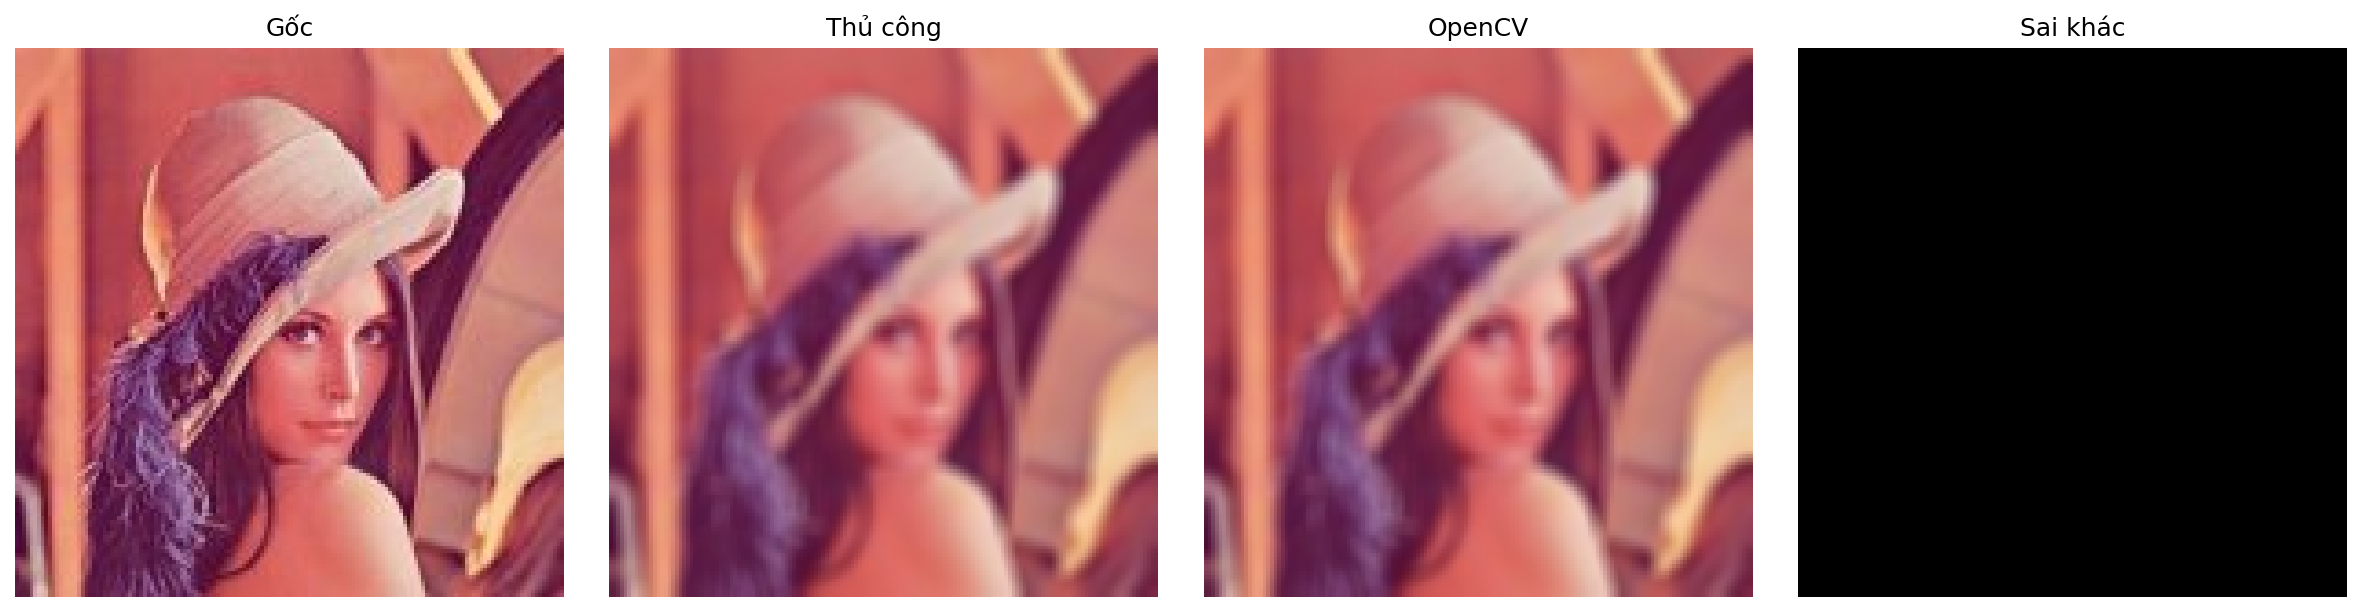
\includegraphics[width=\textwidth]{figures/02_mean_filter.png}
    \caption{So sánh mean filter thủ công và OpenCV.}
\end{figure}

Gaussian filter dùng kernel có trọng số theo phân phối Gaussian. So với mean filter, bộ lọc này thường giữ cấu trúc ảnh mềm và tự nhiên hơn vì pixel gần tâm có ảnh hưởng lớn hơn pixel xa tâm. Kết quả thực nghiệm cho MSE $0.0053$, nghĩa là ảnh thủ công và OpenCV vẫn rất gần nhau nhưng đã có sai khác lớn hơn mean filter do bước tạo kernel, tích chập và làm tròn. Bản thủ công chạy trong $0.222884$s với bộ nhớ đỉnh $802.26$KB, còn OpenCV mất $0.001628$s và $66.35$KB. Ảnh sai khác cho thấy khác biệt chủ yếu xuất hiện nhẹ ở các vùng chuyển mức xám và biên mềm.

\begin{figure}[H]
    \centering
    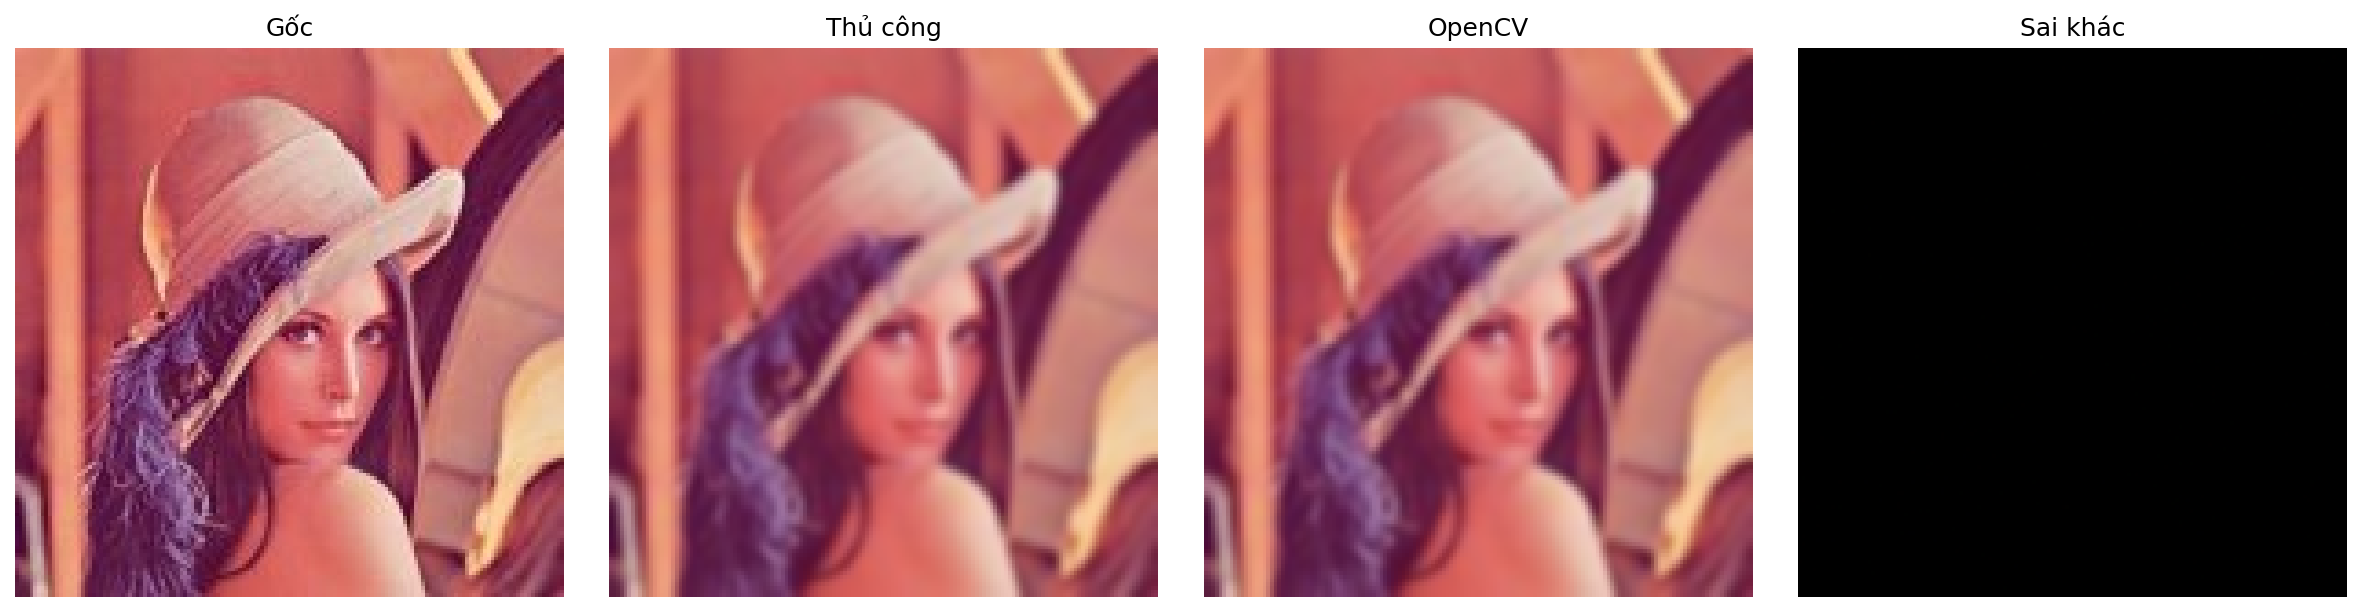
\includegraphics[width=\textwidth]{figures/03_gaussian_filter.png}
    \caption{So sánh Gaussian filter thủ công và OpenCV.}
\end{figure}

Median filter lấy trung vị trong vùng lân cận, do đó có khả năng loại bỏ nhiễu điểm tốt. Kết quả có xu hướng giữ biên tốt hơn mean filter trong một số vùng ảnh. Trong ba phép làm trơn, median filter có sai khác lớn nhất giữa hai cách cài đặt với MSE $0.4045$. Nguyên nhân hợp lý là thao tác lấy trung vị phụ thuộc mạnh vào cách xử lý biên và cách sắp xếp giá trị trong từng cửa sổ. Bản thủ công cần $0.817596$s và $216.54$KB, còn OpenCV chỉ mất $0.000487$s và $66.18$KB, nên đây cũng là phép lọc cho thấy rõ nhất lợi thế tối ưu của thư viện.

\begin{figure}[H]
    \centering
    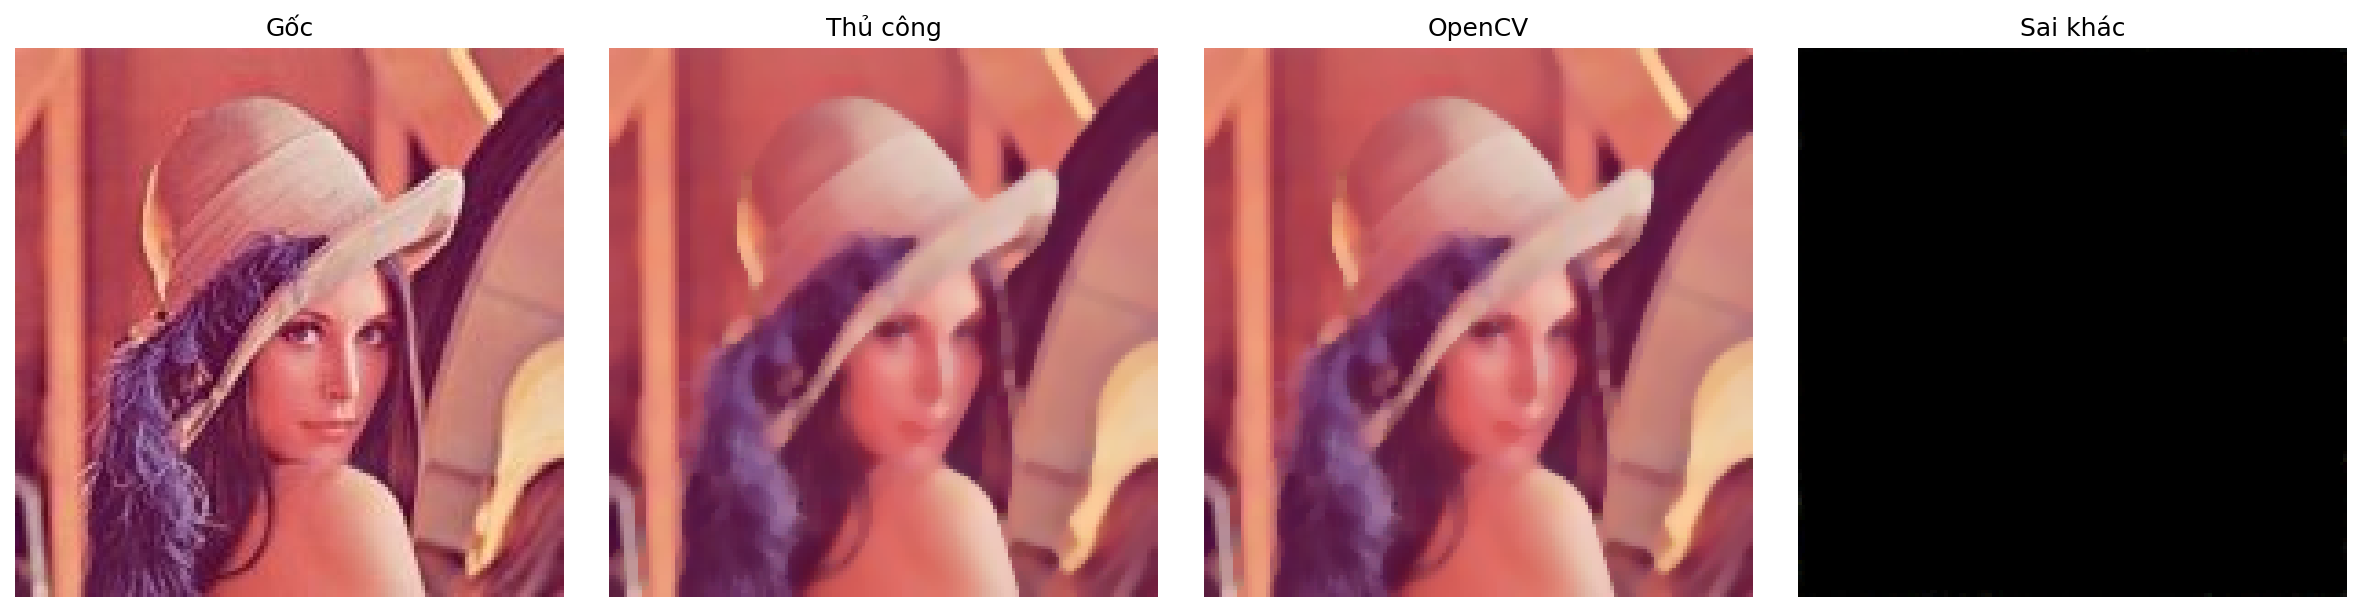
\includegraphics[width=\textwidth]{figures/04_median_filter.png}
    \caption{So sánh median filter thủ công và OpenCV.}
\end{figure}

\subsection{Phát hiện biên cạnh}

Sobel phát hiện biên bằng cách tính gradient theo hai hướng. Ảnh biên thể hiện rõ các vùng thay đổi cường độ sáng như đường viền khuôn mặt, nón và vai áo trong ảnh Lenna.

\begin{figure}[H]
    \centering
    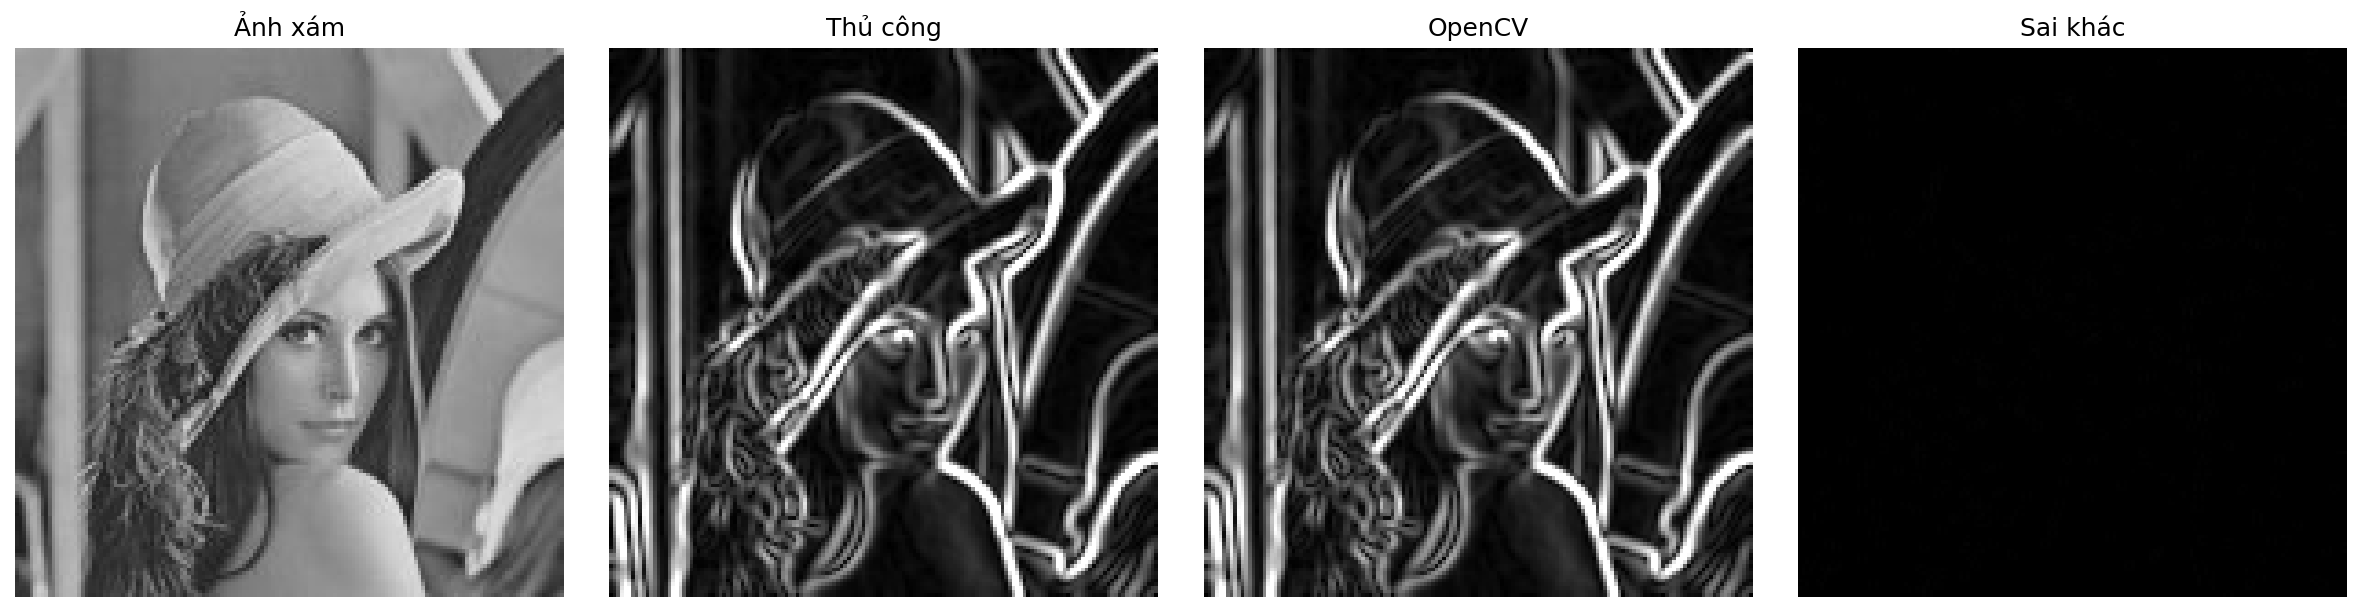
\includegraphics[width=\textwidth]{figures/05_sobel.png}
    \caption{So sánh phát hiện biên Sobel thủ công và OpenCV.}
\end{figure}

Laplacian dùng đạo hàm bậc hai nên phản ứng mạnh tại vùng có thay đổi cường độ đột ngột. Trước khi áp dụng Laplacian, ảnh được làm trơn Gaussian để giảm bớt nhiễu.

\begin{figure}[H]
    \centering
    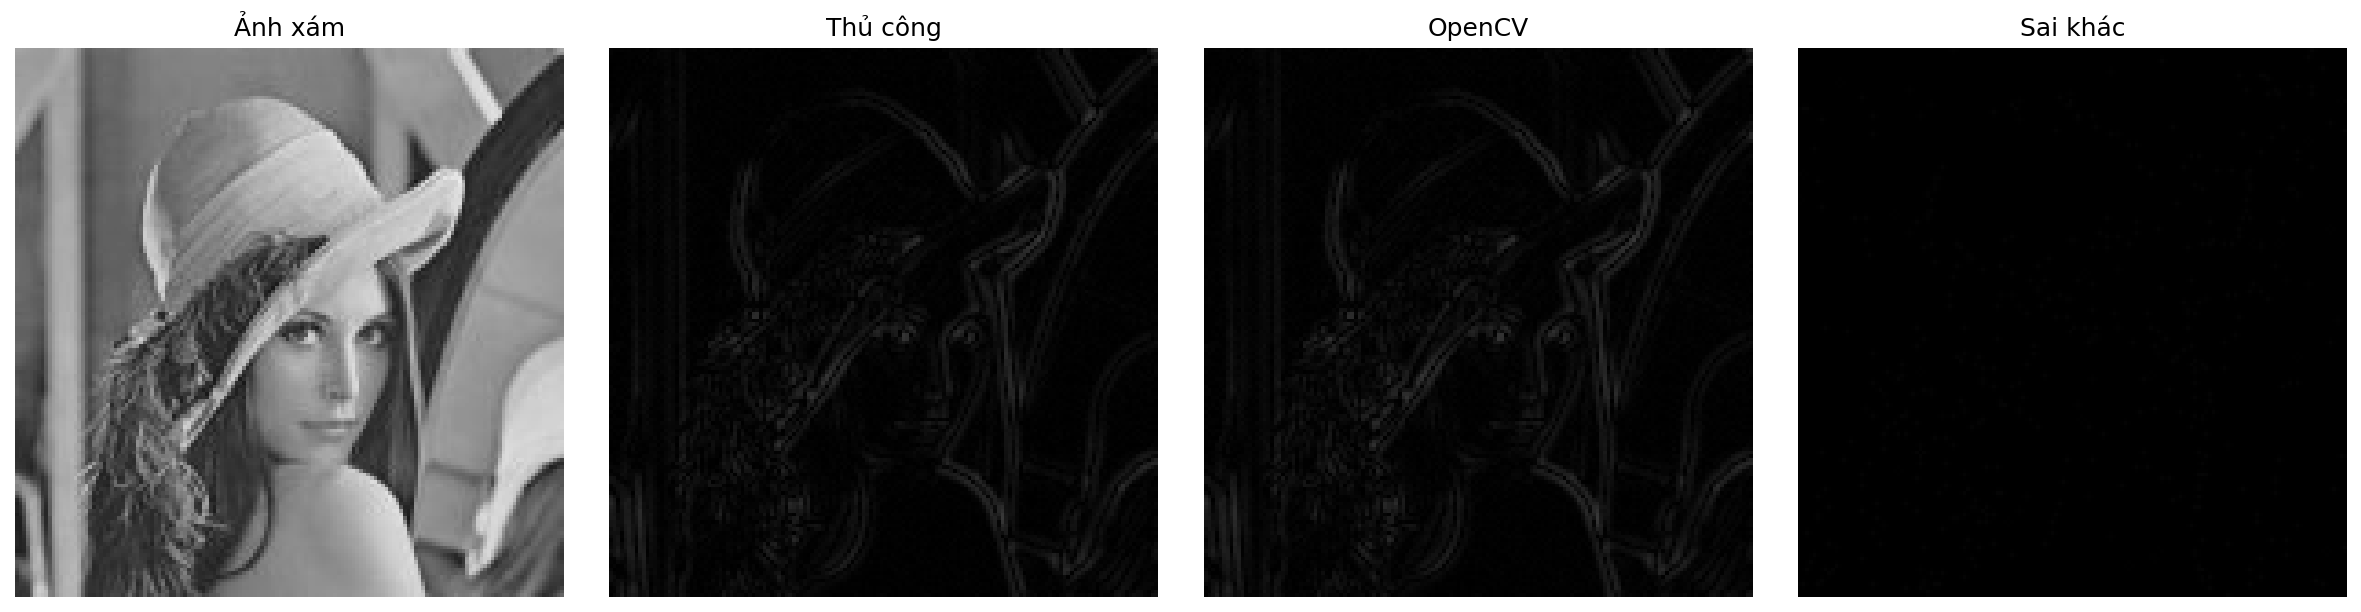
\includegraphics[width=\textwidth]{figures/06_laplacian.png}
    \caption{So sánh phát hiện biên Laplacian thủ công và OpenCV.}
\end{figure}

LoG (Laplace of Gaussian) kết hợp bước làm trơn Gaussian với toán tử Laplacian. Vì vậy, phương pháp này vừa thuộc nhóm phát hiện biên, vừa thể hiện rõ vai trò của bước làm trơn trong việc hạn chế nhiễu trước khi lấy đạo hàm bậc hai. Kết quả đo được cho MSE $72.2126$, cao hơn đáng kể so với Laplacian thường, cho thấy cách cài đặt thủ công và OpenCV khác nhau rõ hơn khi dùng kernel 8-neighborhood và tham số Laplacian của thư viện. Thời gian chạy của bản thủ công là $0.342847$s với $293.61$KB, còn OpenCV mất $0.001922$s và $88.54$KB.

\begin{figure}[H]
    \centering
    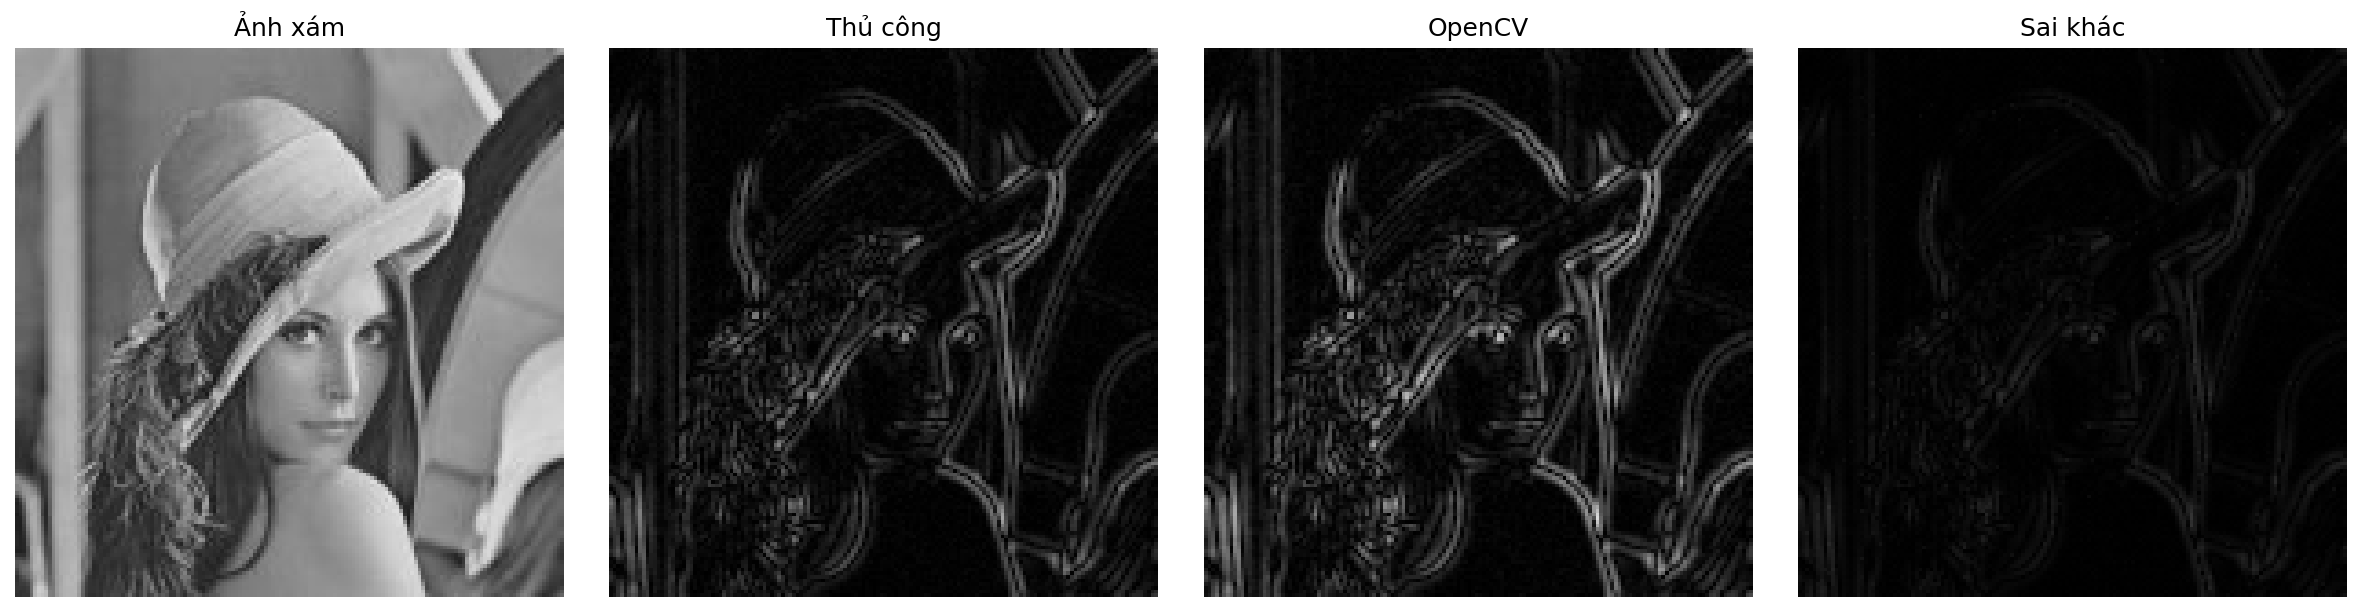
\includegraphics[width=\textwidth]{figures/07_log.png}
    \caption{So sánh phát hiện biên LoG thủ công và OpenCV.}
\end{figure}

Canny tạo biên mảnh hơn nhờ bước non-maximum suppression và ngưỡng kép. Kết quả thủ công có thể khác OpenCV nhiều hơn Sobel và Laplacian vì OpenCV tối ưu nhiều chi tiết nội bộ trong quá trình làm mảnh và nối biên.

\begin{figure}[H]
    \centering
    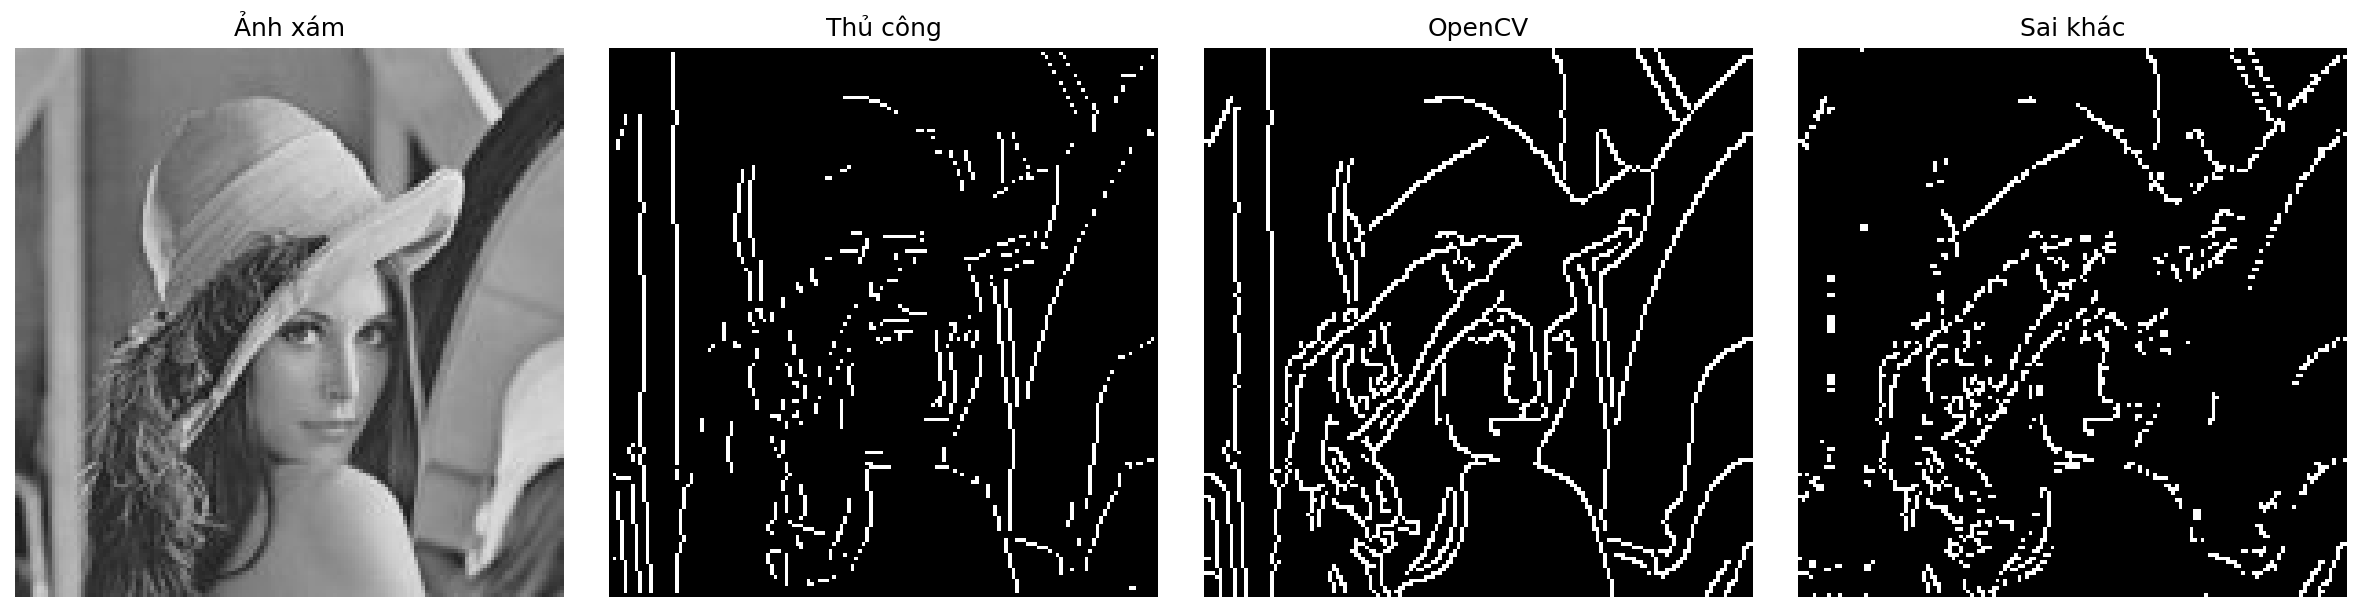
\includegraphics[width=\textwidth]{figures/08_canny.png}
    \caption{So sánh phát hiện biên Canny thủ công và OpenCV.}
\end{figure}

\subsection{So sánh kết quả}

Bảng dưới đây được cập nhật theo kết quả lưu từ lần chạy notebook gần nhất. Nhóm làm trơn gồm ba bộ lọc (mean, Gaussian, median), còn LoG được tính vào nhóm phát hiện biên.

\begin{longtable}{p{0.22\textwidth}p{0.13\textwidth}p{0.18\textwidth}p{0.18\textwidth}p{0.23\textwidth}}
\toprule
\textbf{Phép xử lý} & \textbf{MSE} & \textbf{Thủ công} & \textbf{OpenCV} & \textbf{Nhận xét} \\
\midrule
Mean filter & 0.0000 & 0.365850s | 1080.70KB & \textbf{0.001042s | 66.35KB} & Hai kết quả gần như trùng nhau; ảnh sai khác rất nhỏ và chủ yếu đến từ làm tròn hoặc xử lý biên. \\
Gaussian filter & 0.0053 & 0.222884s | 802.26KB & \textbf{0.001628s | 66.35KB} & Kết quả trực quan vẫn rất gần nhau; sai khác tăng nhẹ do kernel Gaussian và phép tích chập số thực. \\
Median filter & 0.4045 & 0.817596s | 216.54KB & \textbf{0.000487s | 66.18KB} & Median thủ công chậm nhất trong ba phép làm trơn vì phải tính trung vị cho từng cửa sổ ảnh. \\
LoG & 72.2126 & 0.342847s | 293.61KB & \textbf{0.001922s | 88.54KB} & LoG kết hợp làm trơn Gaussian và Laplacian nên nhạy với khác biệt trong kernel và cách hiện thực của OpenCV. \\
Sobel & 0.2713 & 0.511674s | 470.94KB & \textbf{0.001183s | 397.21KB} & Biên chính được phát hiện rõ; sai khác nhỏ có thể do padding và kiểu dữ liệu. \\
Laplacian & 0.3692 & 0.338727s | 293.96KB & \textbf{0.012127s | 88.54KB} & Phản ứng mạnh tại vùng biến thiên cường độ; nhạy với nhiễu nên cần Gaussian trước. \\
Canny & 4629.7798 & 0.560139s | 563.33KB & \textbf{0.003300s | 44.40KB} & Sai khác có thể lớn hơn vì Canny gồm nhiều bước và OpenCV có tối ưu nội bộ. \\
\bottomrule
\end{longtable}

Nhìn chung, cài đặt thủ công giúp hiểu rõ nguyên lý của từng thuật toán, nhưng tốc độ chậm hơn do sử dụng vòng lặp Python. OpenCV phù hợp hơn khi cần xử lý nhanh, ổn định và triển khai thực tế. Trong các kết quả đo được, Mean filter có MSE thấp nhất, còn LoG và Canny cho sai khác lớn hơn do quy trình xử lý phức tạp hơn và phụ thuộc nhiều vào chi tiết hiện thực.

\section{Kết luận}

Bài thực hành hoàn thành hai nhóm nội dung: làm trơn ảnh và phát hiện biên cạnh. Ở phần làm trơn, notebook khảo sát ba bộ lọc gồm mean filter, Gaussian filter và median filter. Các bộ lọc làm trơn giúp giảm nhiễu và chuẩn bị ảnh tốt hơn cho bước phát hiện biên. Các thuật toán phát hiện biên cho thấy nhiều cách tiếp cận khác nhau: Sobel dựa trên gradient bậc một, Laplacian dựa trên đạo hàm bậc hai, LoG kết hợp làm trơn với Laplacian để phát hiện biên, còn Canny gồm nhiều bước để tạo biên mảnh và rõ hơn.

Kết quả so sánh cho thấy OpenCV nhanh hơn đáng kể so với cài đặt thủ công. Tuy nhiên, phần cài đặt thủ công vẫn cần thiết trong bài thực hành vì giúp kiểm chứng công thức, hiểu rõ xử lý kernel, padding, gradient, ngưỡng và quá trình tạo ảnh biên.

\end{document}
